\subsection{Hydrological correction and conversion of the DTM}
An important element of realistic flood modelling is to be able to simulate correct hydrological behaviour through terrain. This requires that the DTM is corrected and converted to a digital hydrological terrain model (named DHyM) in order to be able to use the model result with confidence.\\

To convert a DTM to a DHyM, two hydrological adaptations are used. The adaptations are both polyline geometric objects and are burned into the DTM to simulate correct geographical features in the landscape that have not been captured by the LiDAR scanning.\\

Since adaptations exists for both cloudburst and storm surge applications, it is important to only use those adaptations that have an impact on sea level rise and storm surge modelling. This means that adaptations that are designed, for example, discharge rainwater from cloudbursts into the sea should not be included. Adaptations such as cloudburst no-return valves have therefore been filtered out from the dataset for each area.\\
This is done for both line and horseshoe adaptations using a tool from the Inundation Models toolset called \textit{"Extract Hydroconditioning Inundation"}. First the tool searches for all adaptations within the area boundary. Then, a search is made in the attribute table for a application description. For storm surge modelling, there are three relevant is describe in table \ref{Tabel: Relevante hydrologiske tilpasninger}. The adaptations that meet one of the criteria are transferred to a new layer, one for line and one for horseshoe adaptations. 
\begin{table}[H]
	\centering
	\renewcommand{\arraystretch}{1.5}
	\begin{threeparttable}
		\caption{Relevant hydrological adaptations for storm surge modelling. Source: \cite{GeoDanmark_HydroLag}.}
		\label{Tabel: Relevante hydrologiske tilpasninger}
		\begin{tabular}{@{} l l @{}} 
			\toprule
			\textbf{Adaptation type} & \textbf{Description} \\
			\midrule
			\textit{Generel} &
			\makecell[l]{The normal adaptation of hydrological conditions\\
				(ex creation of free passage under a bridge)} \\
			\addlinespace
			\textit{Sea level rise} &
			\makecell[l]{Adaptations meant to prevent water from entering the land\\
				(ex closure of a water lock)} \\
			\addlinespace
			\textit{DHMFix} &
			\makecell[l]{Used for changes, that a hydrological effect on the\\ free flow of water on the surface\\
				(ex correcting mistakes or oversights in the specific DEM)} \\
			\bottomrule
		\end{tabular}
	\end{threeparttable}
\end{table}

Before the adaptations were burned into the DTM, the horseshoe adaptations were changed from their original horseshoe shape to separate lines between the outer edges of the horseshoe. This is done to have extract size and extent of the adaptation burned into the DTM rather than the outline of the adaptation. This is done using a python script \textit{"Convert Horseshoes to Lines"} where both the line and horseshoe adaptation found in \textit{"Extract Hydroconditioning Inundation"} are converted to separate entities. This conversion makes the calculation of elevation values at the adaptations easier and thus easier to burn into the DTM.\\
To create the individual lines from the horseshoes the four corner points and the DTM's cell size were used. The visual transformation is shown in figure \ref{Figur: Ændringen af hesteskotilpasningerne}. Where figure \ref{Subfig: Hesteskotilpasninger før ændring} is the adaptation before transformation and figure \ref{Subfig: Hesteskotilpasning efter tilpasningen er konverteret til linjer} is the adaptation after conversion. Each line is exactly one cell size wide (40 cm), as larger line width is not necessary in order to simulate hydrological movement through the terrain.
\begin{figure}[H]
	\begin{subfigure}[t]{0.5\textwidth}
		\centering
		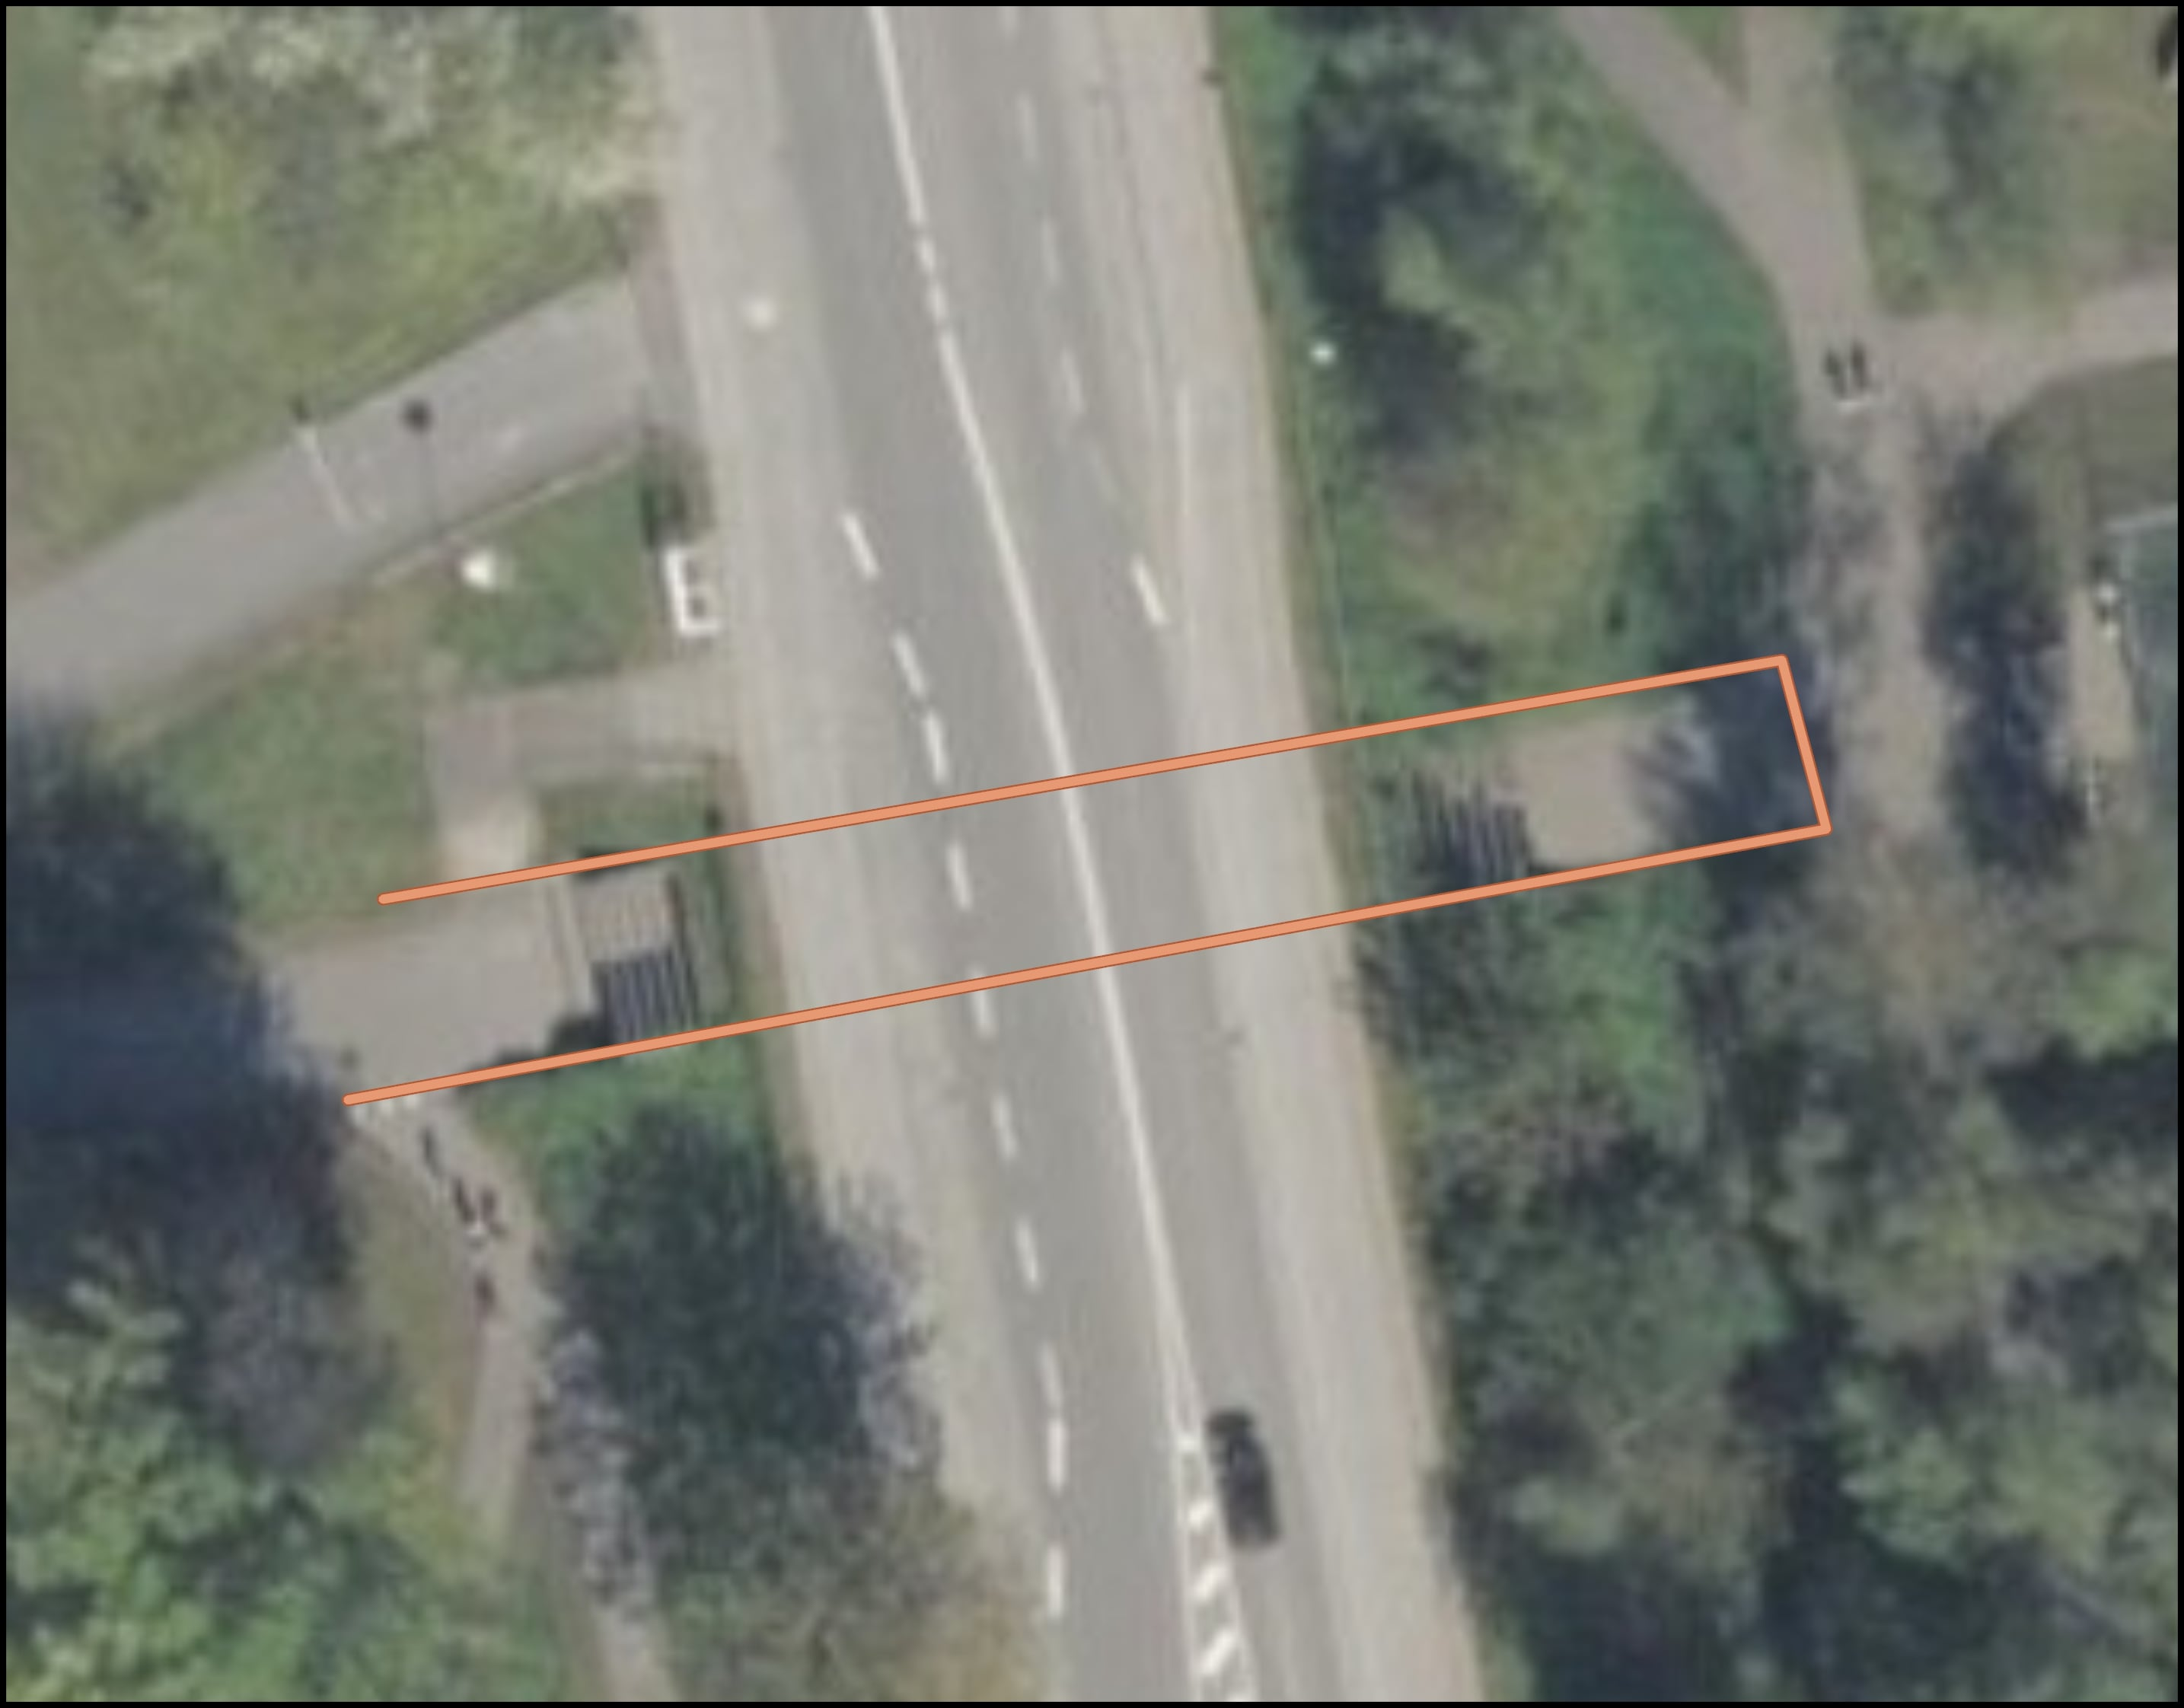
\includegraphics[width=1\linewidth]{images/databeskrivelse/hestesko.jpg}
		\caption{}
		\label{Subfig: Hesteskotilpasninger før ændring}
	\end{subfigure}
	\hspace{0.2cm}
	\begin{subfigure}[t]{0.5\textwidth}
		\centering
		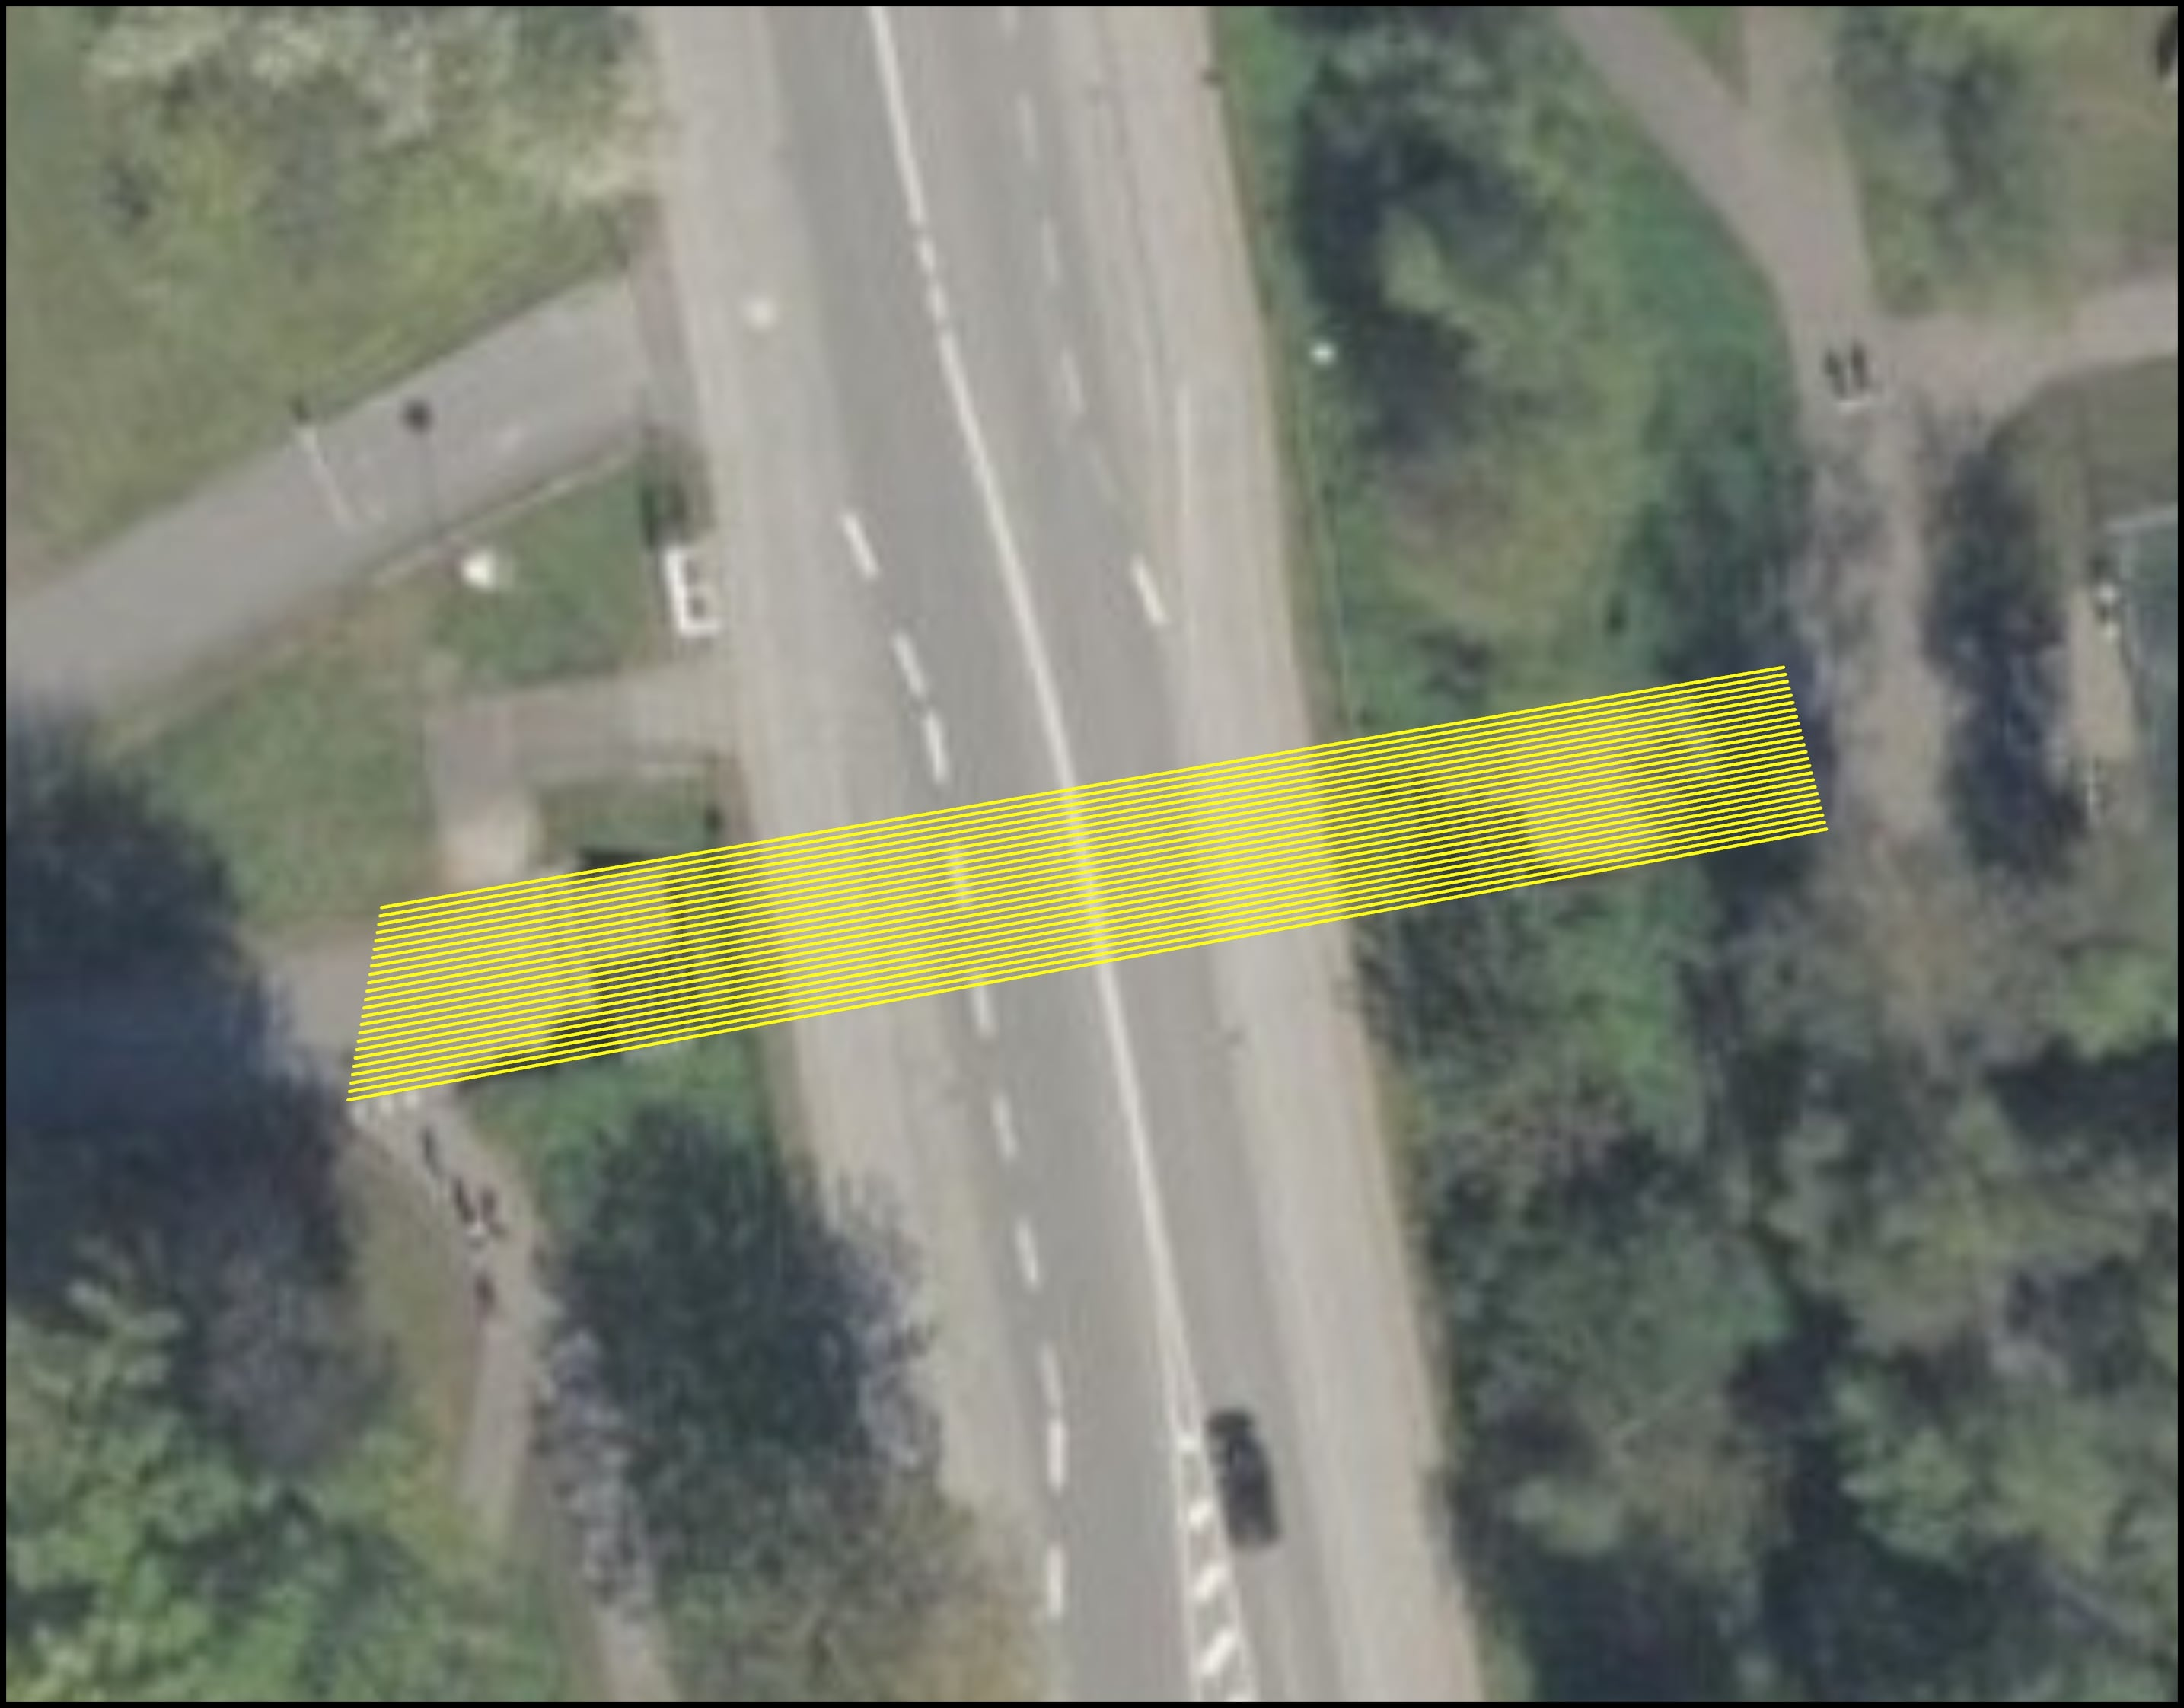
\includegraphics[width=1\linewidth]{images/metode/hestesko_linjer.jpg}
		\caption{}
		\label{Subfig: Hesteskotilpasning efter tilpasningen er konverteret til linjer}
	\end{subfigure}
	\caption{Ændringen af en hesteskotilpasning fra en hesteskoform til separate linjer. \textbf{(a)} Hesteskotilpasningen før ændring. \textbf{(b)} Hesteskotilpasningen efter tilpasningen er konverteret til separate linjer.}
	\label{Figur: Ændringen af hesteskotilpasningerne}
\end{figure}

This creates a new merged layer with all the relevant adaptations in a polyline format. In order for the adaptations to be represented in the DHyM, elevation values under terrain obstacles must first be interpolated and assigned to each adaptation.\\
This was done using another python script \textit{"Hydrologic Conditioning Multiple} \citep{balstrom_identification_2024}. The script assigns a z-value from the DTM to each of the line endpoints: $Z_0$ and $Z_1$. From the line endpoints, the line slope, $\Delta{Z}$, is calculated using the distance between the endpoints. The line is then converted into a raster format and then to a point format. For each cell in the DTM, a point is placed on the line. Then, a linear interpolation of the points along the line is performed based on the starting point $Z_0$, the distance from $Z_0$ to a point and the line slope, $\Delta{Z}$. This is done for all points along the line (figure \ref{Figur: Interpolation af Z-værdier}).\\

After the z-values have been interpolated, the points are converted back into a raster format, after which the adaptations are burned into the DTM by combining the interpolated cells with the DTM. The combination is done by checking for NoData cells in the point raster. If the value is NoData, then z-values from the DTM are used. If the value is not NoData, then the z-value in the DTM is replaced with the corresponding z-value in the point raster.
Together this establishes the corrected digital hydrological terrain model (DHym).

\begin{figure}[H]
	\centering
	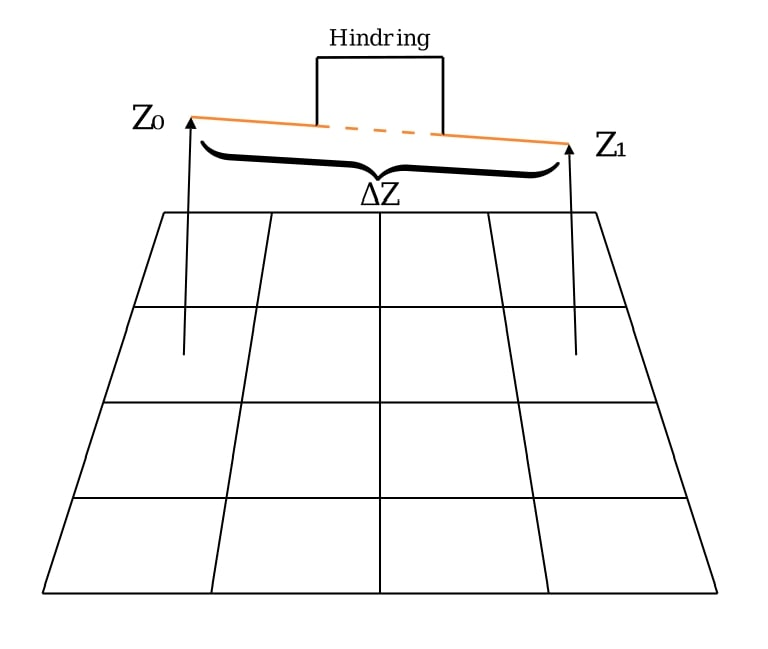
\includegraphics[width=0.5\linewidth]{images/metode/dtm_hydro_z.jpg}
	\caption{Interpolationen af z-værdier langs den orange linje for en linjetilpasning under en hindring. $Z_1$ og $Z_0$ er z-værdierne fra DTM ved linjetilpasningens endepunkter og $\Delta{Z}$ er hældningen af linjetilpasningen. Egen illustration med inspiration fra \cite{balstrom_identification_2024}.}
	\label{Figur: Interpolation af Z-værdier}
\end{figure}
For Aabenraa, Gedser Havn, Hesnæs and Præstø: 250, 13, 34, and 19 relevant hydrological adaptations were identified and burned into their associated DTM.

\subsubsection{Inclusion of buildings}
As an extra measure for simulating correct water behaviour through the terrain, it was decided to include building footprints in the DHyM as impermeable barriers. This decision was based on the fact that the flood maps provided from the study sites treated buildings as barriers. Furthermore, it was assessed that realistic simulation of water movement assumes that water cannot flow directly through buildings, but is diverted around them.\\

The method for implementing buildings in the DHyM done using the \textit{"Building Block (BB)"} method used in \cite{khosh_bin_ghomash_technical_2024}. This method raises the terrain values in the elevation model for each building polygon's footprint to a certain height. This height was arbitrarily set to 20 metres for all buildings. The building polygons were then converted to a raster format with a cell size of 0.4\times0.4 metres.\\
A check is then performed on the new building raster, where cells that contain a value of 20, remains 20 and cells with NoData were assigned 0. This ensure that the building raster can be combined correctly with the DHyM, since mathematical expressions using NoData are not possible. Finally, the building raster and DHyM were added together, creating the final iteration of the DHyM used in the Inundation Model.

\subsubsection{Modelling the 2023-storm surge event}\label{Afsnit: Simulering af stormflod 2023}
With a processed DHyM it is possible to model the storm surge event in 2023 using the Inundation Model. In the models GUI, the corresponding DHyM and line source \textit{"Line At Sea"} are inputted for each area. The Line at Sea is a manually digitized line at a random location in the sea. \\
Each area is modelled up to the highest official water level recorded during the event and the number of iterations to achieve this level is shown in \ref{Tabel: Antal iterationer og slutværdier for Inundation Model}. All areas begin the flood modelling with a starting value of 100 centimetres and an increment value of 1 centimetre. A starting value of 100 centimetres was chosen primarily to reduce processing time and the increment value of 1 centimetre was chosen to achieve the greatest flexibility. The processing duration for each area is shown in \ref{Tabel: Antal iterationer og slutværdier for Inundation Model} and it took 12 hours and 1 minute to process all areas in total on a Lenovo i5-6500T 2.5GHz CPU with four cores and processors and 16GB of RAM.\\





\begin{table}[H]
	\centering
	\renewcommand{\arraystretch}{1}
	\begin{threeparttable}
		\caption{Number of iterations, end value, and processing duration for inundation modelling using th Inundation Model for the October 2023 storm surge event}
		\begin{tabular}{@{} l 
				S[table-format=7.2, output-decimal-marker={,}] 
				S[table-format=7.2, output-decimal-marker={,}]
				l @{}} 
			\toprule
			\textbf{Location} & \textbf{Iterations} & \textbf{End Value (cm)}  & \textbf{Processing duration}\\
			\midrule
			Aabenraa & 117 & 216 & 5 hours 27 minutes \\
			Gedser & 90 & 189 & 3  hours 25 minutes\\ 
			Hesnæs & 111 & 210 & 1 hour 23 minutes \\
			Præstø & 101 & 200 & 1 hour 44 minutes \\
			\bottomrule
		\end{tabular}
		\label{Tabel: Antal iterationer og slutværdier for Inundation Model}
	\end{threeparttable}
\end{table}
After the simulation was complete, a raster is produced for each centimetre until the end value. An internal ArcGIS Pro tool \textit{"Cell Statistics"} was then used to find the minimum value that a given cell would be inundated and combine all rasters into a single raster. This raster was then filtered with a land polygon so only cells on land were part of the result. This is done because the model technically finds possible inundated cells on sea because those cells are equal to 1 in the SetNull function. By using the land polygon those extra unnecessary values are removed from the final result.\\

\subsubsection{Statistical 100-year events and a projection of the 2023 storm surge event}
In light of future climate change the risk of rising sea levels in Denmark, an investigation of how two types of projected storm surge events in the future might impact the study sites. The two events are: a statistical water level for a 100-year storm surge event and a projection of what the 2023 storm surge will look like in the year 2100 based on sea level rise projections from the sixth \cite{ipcc_report_AR6} report. For both events types, two different Shared Socioeconomic Pathways (SSP) scenarios are simulated: a medium-high emission scenario (SSP2-4.5) and a very high emission scenario (SSP5-8.5). The medium-high scenario was chosen as a compromise-based middle position between the highest possible emission scenario and the mildest, although \cite{dmi_ny_nodate} emphasizes that municipalities and management stakeholders should use the high emission scenario (SSP3-7) in climate assessments. The very high scenario was chosen to simulate an event under the worst possible outcome.\\ 

\noindent
\textit{Statistical 100-year event}\\
To analysis the impact of a statistical 100-year storm surge had on the areas, DMI's Climate Atlas was used to determine the sea level of storm surge that will statistically occur once per 100 years. The Climate Atlas divides Denmark's coasts into coastal stretches and the four coastal stretches used are: Lillebælt South for Aabenraa, Fehmarnbælt for Gedser, Falster and Møn's Baltic Sea coast for Hesnæs and Faxe Bugt for Præstø- For each coastal stretch, the absolute sea level for a 100-year event at SSP2.5-4.5 and SSP55-8.5 is used.\\

The Inundated Model is then used to simulate up to the SSP5-8.5 scenario. The process is the same as in section \ref{Afsnit: Simulering af stormflod 2023}, but instead of starting at 100 centimetres, the model starts at the last iterated sea level. The model simulated up to 251 cm for Aabenraa, 242 cm for Gedser, 253 cm for Hesnæs and 225 cm for Præstø and adding an extra 2 hours and 46 minutes in total processing duration.\\

\noindent
\textit{Projection of the 2023 storm surge event}\\
Since the sea level in Denmark is expected to rise during the current century, it has therefore been desired to investigate how the 2023 storm surge event would impact the study sites if it occurred at the end of the current century. To do this, a calculation of the mean sea level in 2100 has been made. DMI's Climate Atlas already has values for the mean sea level in 2100, but their values are relation to a reference period from 1981-2010. It has therefore been necessary to calculate the mean sea level in 2023 in relation to DMI's reference period then calculate the mean sea level in 2100 based on the sea level in 2023.\\

To perform this calculation, a dataset from \cite{garner_ipcc_2021} of sea level projections and an online tool developed by NASA \citep{NASA_tool} have been used. NASA's tool makes it possible t obtain projections for a specific Permanent Service for Mean Sea Level (PSMSL) station. The tool selects the nearest PSMSL station for each area. The station was chosen based on which ocean basin was the closest to each area. This was Fynshav for Aabenraa, Gedser Havn for Gedser, Warnemünde for Hesnæs and Skanör for Præstø.\\

The tool then provides a table with all the individual contributions to sea level rise and a median sea level rise ($SLR_{50}$) for each station relative to a reference period from 1995-2014. $SLR_{50}$ includes factors such as freshwater input from rivers, glacial contributions and local isostasy. To calculate the mean sea level in 2023, the projection for 2030 has been used, as it is the closest year. For the calculation, the following equation has been established:
\begin{align} \label{Equation: Vandstandsstigning calculation}
	S_r = S_p- \left( \frac{\Delta{t}}{\Delta{t_r}}\times SLR_{50} + \Delta{M_r} \times \left(\frac{SLR_{50}}{\Delta{t_r}}\right) \right)
\end{align}
The mean sea level in 2023 is then calculated by finding the ratio of the difference between the target year 2023 ($\Delta{t}$), NASA's reference year ($\Delta{t_r}$) and the projection year (2030). This ratio is then multiplied by $SLR_{50}$ and gives the mean sea level in 2023 relative to NASA's reference period (1995-2014). The expected mean sea level increase from DMI's reference period (1981-2010) to NASA's reference periodis then calculated. This calculation is made under the assumption that the increase from DMI's to NASA's reference period has been linear \citep{danish_meteorological_institute_dmi_2024}.This is done by taking the difference between the median years of each reference periods ($\Delta{M_r}$) and multiplying the rate of sea level rise ($\frac{SLR_{50}}{\Delta{t_r}}$) up to 2023.\\
This gives a result for what the mean sea level in 2023 has been in relation to the DMI reference period and makes it possible to subtract this sea level value from the projected sea level in 2100 ($S_p$) and gives $S_r$, which is the mean sea level in 2100 with 2023 as the new reference year. This procedure was carried out for a SSP2-4.5 and SSP5-8.5 scenario.\\

The Inundation Model was then run again to obtain new flooding extend maps. Up to 268 centimetres for Aabenraa, 259 for Hesnæs and 246 for Præstø. No new storm surge level was modelled for Gedser as the 100-year event at SSP8.5 is a higher sea level rise than the projected storm surge level in 2100. The projections added an additional 1 hour and 58 minutes to the total processing duration.\\

Then all the inundation rasters were converted to a polygon format and combined with the tool \textit{"Merge"} to visualise flooding extent from both 100-year event and the projections on a single map.
